\documentclass[a4paper,titlepage]{article}

\makeatletter
\def\input@path{{../../../template/}{./img}}
\makeatother

\usepackage{Comandi}
\usepackage{Stile}
\usepackage{Riferimenti}

 
 \def\NOME{Norme di Progetto}
 \def\VERSIONE{0.1}
 \def\DATA{\today}
 \def\REDATTORE{Matteo Franco\\ & Luca Soldera}
 \def\VERIFICATORE{Enrico Bellio}
 \def\RESPONSABILE{Viviana Alessio}
 \def\USO{Interno}
 \def\DESTINATARI{\COMMITTENTE \\ & \CARDIN \\ & \PROPONENTE}
 \def\SOMMARIO{Questo documento definisce le norme stabilite dal gruppo Beacon Strips per la realizzazione del progetto CLIPS}
 
\begin{document}
\maketitle

\begin{diario} %dal 3-3 al 15-3
	
	\modifica{Luca Soldera}{\AM}{Correzione sezione Repository relativa al Processo di gestione)}{2016-03-09}{0.5.2}
	\modifica{Matteo Franco}{\AM}{Correzione sezione Norme relativa al Processo di documentazione}{2016-03-09}{0.5.1}
	\modifica{Luca Soldera}{\AM}{Stesura sezioni Procedure e Norme relative al Processo di gestione}{2016-03-08}{0.6.0}
	\modifica{Matteo Franco}{\AM}{Stesura sezioni Attività e Strumenti relative al Processo di gestione}{2016-03-07}{0.5.0}
	\modifica{Luca Soldera}{\AM}{Stesura sezione Processi primari}{2016-03-06}{0.4.0}
	\modifica{Matteo Franco}{\AM}{Completamento stesura sezione Processo di documentazione}{2016-03-06}{0.3.0}
	\modifica{Luca Soldera}{\AM}{Stesura sezione Processo di verifica}{2016-03-04}{0.2.1}
	\modifica{Matteo Franco}{\AM}{Inizio stesura sezione Processo di documentazione}{2016-03-04}{0.2.0}
	\modifica{Matteo Franco}{\AM}{Creazione scheletro documento e stesura sezione Introduzione}{2016-03-03}{0.1.0}
\end{diario}
 
 %aggiungere a norme di progetto regole su:
 %ordine indici: prima argomenti, poi tabelle, poi immagini
 %verbali: template e struttura
 %aggiungere formato orario e formato indirizzo
 
\newpage

\tableofcontents

\section{Introduzione}
	\subsection{Scopo del documento} 
	Questo documento ha lo scopo di spiegare dettagliatamente le strategie secondo cui il gruppo \AUTORE{} intende condurre il \gl{progetto} didattico. 
	\subsection{Scopo del \gl{prodotto}}
	\SCOPO
	\subsection{Glossario}
	\GLOSSARIO
	\subsection{Riferimenti}
		\subsubsection{Normativi}
			\begin{itemize}
				\item \textbf{Capitolato d'appalto C2 - CLIPS:} Communication \& Localisation with Indoor Positioning Systems. \\
				\url{http://www.math.unipd.it/~tullio/IS-1/2015/Progetto/C2.pdf}
				\item \textbf{Vincoli e dettagli tecnico-economici} \\
				\url{http://www.math.unipd.it/~tullio/IS-1/2015/Dispense/PD01.pdf}
				\item \textbf{Norme di Progetto} \\ \NPdoc
				\item \textbf{Regolamento di Progetto} \\
				\url{http://www.math.unipd.it/~tullio/IS-1/2015/Progetto/}
				\item \textbf{Regolamento organigramma} \\
				\url{http://www.math.unipd.it/~tullio/IS-1/2015/Progetto/PD01b.html}
			\end{itemize}	
			
		\subsubsection{Informativi}
			\begin{itemize}
				\item \textbf{Software Engineering (10th edition}) \\
				Ian Sommerville \\
				Pearson Education | Addison-Wesley
				\item \textbf{Guide to the Software Engineering Body of Knowledge}
				IEEE Computer Society. Software Engineering Coordinating Committee
				\item \textbf{Slides del \COMMITTENTE} \\ riguardo i  \href{http://www.math.unipd.it/~tullio/IS-1/2015/Dispense/L02.pdf}{processi \gl{software}}, il \href{http://www.math.unipd.it/~tullio/IS-1/2015/Dispense/L03.pdf}{ciclo di vita del \gl{software}} e \href{http://www.math.unipd.it/~tullio/IS-1/2015/Dispense/L04.pdf}{la gestione di \gl{progetto}}	
			\end{itemize}
	\subsection{Modello di ciclo di vita scelto}
	È stato scelto come ciclo di vita il modello \gl{incrementale}. Le motivazioni che ci hanno spinto verso questa direzione sono il modo in cui è strutturato il \gl{progetto} didattico e la quasi totale inesperienza dei componenti del gruppo nello sviluppare progetti \gl{software} di grandi dimensioni. Di seguito una lista di caratteristiche del metodo \gl{incrementale}:
	\begin{itemize}
		\item si può produrre valore ad ogni incremento;
		\item ogni incremento riduce il rischio di fallimento;
		\item prevede rilasci multipli;
		\item i requisiti utente sono classificati e trattati in base alla loro importanza strategica. I requisiti più importanti sono già stabili all'inizio dello sviluppo del \gl{progetto};
		\item l'analisi dei requisiti e la progettazione architetturale non vengono ripetute;
		\item prima si pensa allo sviluppo dei requisiti essenziali, poi a quelli desiderabili;
		\item Sono presenti delle iterazioni del tipo Prototipo $\rightarrow$ Validazione $\rightarrow$ Prototipo $\rightarrow$ Validazione $\rightarrow$ ecc..
	\end{itemize}
	\subsection{Scadenze}
	Il gruppo Beacon Strips ha deciso di rispettare le seguenti scadenze:
	\begin{itemize} 
		\item \textbf{Revisione dei Requisiti}: 2016-04-18
		\item \textbf{Revisione di Progettazione}: 2016-06-17
		\item \textbf{Revisione di Qualifica}: 2016-08-24
		\item \textbf{Revisione di Accettazione}: 2016-09-12
	\end{itemize}
	In base a queste scadenze e a fronte dell'analisi dei rischi verranno decise le fasi in cui suddividere il lavoro di sviluppo del \gl{progetto}.
	\subsubsection{Scelta Revisione di Progettazione}
	Si è deciso di affrontare la RP$_{\mbox{\textit{min}}}$. Il gruppo si impegna quindi per il 2016-06-17 di presentare nel documento ``Specifica Tecnica'' la progettazione ad alto livello del \gl{prodotto}.
	

\section{Processi primari} 
	\subsection{Processo di sviluppo}
		\subsubsection{Attività}
		\paragraph{Analisi dei requisiti}
		Sarà compito degli analisti redigere l'analisi dei requisiti in seguito a riunioni interne col team e allo studio dei capitolati d'appalto.
			\subparagraph{Studio di Fattibilità e Analisi dei Rischi}
			Lo studio di fattibilità sarà il primo documento dell'analisi dei requisiti che analizzerà i seguenti punti per ogni capitolato, con maggior interesse per quello scelto dal team:
			\begin{itemize}
				\item \textbf{Scopo del progetto}: analisi delle richieste del capitolato;
				\item \textbf{Studio del dominio}: valutazione delle tecnologie e conoscenze richieste rispetto l'attuale livello del team;
				\item \textbf{Analisi dei rischi}: ricerca dei rischi e delle criticità per ciascun capitolato.
			\end{itemize}
			\subparagraph{Analisi dei requisiti}
			Il secondo documento che gli analisti andranno a redigere sarà l'analisi dei requisiti che produrrà dei requisiti semplici a partire dalle informazioni raccolte tramite lo studio del capitolato e riunioni esterne con il proponente.
			Per rendere più precisa e veloce la stesura dei requisiti è stato utilizzato il software \gl{Trender}.
	\subsubsection{Norme}
		\paragraph{Classificazione  dei requisiti}
		I requisiti saranno rappresentati secondo la seguente codifica:
		\begin{center}
			R[importanza][tipo][identificativo]
		\end{center}
		\begin{itemize}
			\item \textbf{Importanza}:indica se il requisito è:
			\begin{enumerate}
				\item \textbf{0}: obbligatorio;
				\item \textbf{1}: desiderabile;
				\item \textbf{2}: opzionale.
			\end{enumerate}
			\item \textbf{Tipo}: indica se è di tipo:
			\begin{enumerate}
				\item \textbf{F}: funzionale;
				\item \textbf{Q}: di qualità;
				\item \textbf{P}: prestazionale;
				\item \textbf{V}: di vincolo.
			\end{enumerate}
			\item \textbf{Identificativo}: è il codice univoco e gerarchico che automaticamente il software assegna al requisito(esempio: 4.2.1);
			\item \textbf{Descrizione}: una breve descrizione del requisito;
			\item \textbf{Fonte}: la fonte da cui deriva il requisito.
		\end{itemize}
		\paragraph{Classificazione dei casi d'uso}
		I casi d'uso saranno rappresentati secondo la seguente codifica:
		\begin{center}
			UC[identificativo]
		\end{center}
		\begin{itemize}
			\item \textbf{Identificativo}: codice univoco e gerarchico che automaticamente il software assegna al caso d'uso (esempio: 3.4.1);
		\end{itemize}
		inoltre i casi d'uso saranno caratterizzati da:
		\begin{itemize}
			\item \textbf{Tipo}: se non specificato è di tipo standard altrimenti viene scelto fra:
			\begin{enumerate}
				\item \textbf{estensione};
				\item \textbf{inclusione};
				\item \textbf{generalizzazione}.
			\end{enumerate}
			\item \textbf{titolo} breve del caso d'uso;
			\item \textbf{descrizione} del caso d'uso;
			\item \textbf{precondizione} del caso d'uso;
			\item \textbf{postcondizione} del caso d'uso 
			\item \textbf{scenario principale} degli eventi;
			\item \textbf{scenario secondario} eventuale;
			\item \textbf{attori}: lista degli attori coinvolti;
		\end{itemize}
\subsubsection{Strumenti}
	\paragraph{Trender}
	Per velocizzare e automatizzare la stesura dei requisiti e dei casi d'uso è stato utilizzato il software \textbf{Trender} sviluppato da Simone Campagna del gruppo InfiniTech dell'anno 2014/2015. Il software permette di tracciare i requisiti e i casi d'uso assegnando automaticamente un codice univoco che rispetti la sintassi desiderata.
		
\section{Processi di supporto}
	\subsection{Processo di documentazione}
		\subsubsection{Procedure}
	\paragraph{Ciclo di vita}
	Ogni documento può trovarsi in tre fasi differenti:
	\begin{itemize}
		\item \textbf{In lavorazione}: un documento è in lavorazione quando vengono aggiunti, modificati o rimossi dei contenuti;
		\item \textbf{Da verificare}: quando un documento è completo dovrà essere preso in consegna dai verificatori, che si occuperanno di rilevare e/o correggere errori sintattici e semantici;
		\item \textbf{Approvato}: un documento, ultimata la verifica, deve essere approvato dal \RES. L'approvazione determina lo stato finale della versione del documento.
	\end{itemize}
	Le varie fasi vengono scandite dal sistema di ticketing (vedi sezione 4.1.1.3).
\subsubsection{Norme}
	\paragraph{\gl{Template}}
	È presente una cartella nel \gl{repository} in \file{/documenti/template}. \\
	La cartella contiene i seguenti files:
	\begin{itemize}
		\item \textit{Comandi.sty}: contiene i comandi personalizzati (ad es. \texttt {\textbackslash gl});
		\item \textit{Riferimenti.sty}: all'interno del file sono presenti vari comandi da utilizzare come scorciatoie (ad es. \texttt{\textbackslash RES)};
		\item \textit{Stile.sty}: contiene gli stili grafici da applicare al \gl{template};
		\item \textit{TemplateDoc.tex}: è il \gl{template} da utilizzare per realizzare i documenti. Ogni documento dovrà essere realizzato a partire da questo file;
		\item \textit{TemplateVerbale.tex}: questo \gl{template} va impiegato per realizzare i verbali. Ogni verbale dovrà essere realizzato a partire da questo file;
		\item \textit{Glossario.sty}: questo file serve per impostare il \textit{Glossario}, che avrà una configurazione diversa dal \gl{template} standard. %controllare
	\end{itemize}
	È presente inoltre una cartella \textit{img} dove si trova il logo del team e dove potranno essere caricate tutte le altre immagini necessarie al \gl{template}. 
	\paragraph{Norme tipografiche}
	In questa sezione vengono definite le norme riguardanti l'ortografia e la tipografia, al fine di avere uno stile uniforme per tutti i documenti prodotti.
	\subparagraph{Stile del testo}
		\begin{itemize}
			\item \textbf{Grassetto}: il grassetto va utilizzato nei seguenti casi:
			\begin{itemize}
				\item titoli;
				\item elenchi puntati: può essere utilizzato il grassetto nel caso sia necessario evidenziare il concetto da sviluppare;
				\item altri casi: per evidenziare parole chiave o contenuti importanti.
			\end{itemize}
			\item \textbf{Corsivo}: lo stile corsivo si applica a:
			\begin{itemize}
				\item documenti;
				\item abbreviazioni.
			\end{itemize}
			\item \gl{\LaTeX}: ogni occorrenza di \gl{\LaTeX}{} va scritta con il comando \texttt{\textbackslash LaTeX}
			\item Maiuscolo: è possibile utilizzare lo stile maiuscolo \textbf{solo} per gli acronimi;
			\item \gl{Monospace}: le porzioni di testo scritte in \gl{monospace} definiscono:
			\begin{itemize}
				\item frammenti di codice;
				\item comandi;
				\item URL.
			\end{itemize} 
			\item Glossario: le parole che hanno un riferimento nel glossario sono in corsivo e hanno una 'g' a pedice.
		\end{itemize}
	\subparagraph{Punteggiatura}
		\begin{itemize}
			\item \textbf{Spaziature}: ogni simbolo di punteggiatura deve essere seguito da uno spazio, e mai preceduto;
			\item \textbf{Parentesi}: le parentesi costituiscono un'eccezione riguardo le spaziature, in quanto devono essere precedute da uno spazio, ma non seguite;
			\item \textbf{Virgolette singole}: le virgolette singole indicano un singolo carattere;
			\item \textbf{Virgolette doppie}: le virgolette doppie vanno utilizzate per indicare citazioni e documenti.
		\end{itemize}
	\subparagraph{Composizione del testo}
		\begin{itemize}
			\item \textbf{Elenchi puntati}: ogni punto dell'elenco termina con un punto e virgola, ad eccezione dell'ultimo che deve terminare con un punto fermo. \\
			Ogni punto inizia con la minuscola, tranne nel caso in cui necessiti di una spiegazione: allora si utilizzerà la maiuscola;
			\item \textbf{Nota a piè di pagina}: ogni nota inizia con l'iniziale della prima parola maiuscola e termina con il punto. Non ci sono spaziature tra il numero della nota e il testo.
		\end{itemize}
	\subparagraph{Formati}
		\begin{itemize}
			\item \textbf{Date}: per le date va utilizzata la notazione definita dallo standard \gl{ISO} 8601:2004:
			\highlight{\textit{AAAA -- MM -- GG}}
			dove:
			\begin{itemize}
				\item AAAA: rappresenta l'anno utilizzando quattro cifre;
				\item MM: rappresenta il mese utilizzando due cifre;
				\item GG: rappresenta il giorno utilizzando quattro cifre.
			\end{itemize}
			\item \textbf{Orari}: gli orari rappresentati dovranno essere in linea con lo standard \gl{ISO} 8601:2004:
			\highlight{\textit{HH:MM}}
			dove:
			\begin{itemize}
				\item HH: rappresenta l'ora utilizzando due cifre;
				\item MM: rappresenta i minuti utilizzando due cifre.
			\end{itemize}
			\item \textbf{Indirizzi}: per gli indirizzi verrà utilizzata la rappresentazione:
			\highlight{\textit{Destinatario o luogo - Via e numero, CAP, Comune(Provincia)}}
			Nel caso l'indirizzo si riferisca ad uno Stato estero sarà necessario aggiungere il nome dello Stato dopo la provincia.	
			\item \textbf{Sigle}: le sigle dei documenti vanno utilizzate solo nei diagrammi o nelle tabelle, con lo scopo di risparmiare spazio. Tali sigle sono:
			\begin{itemize}
				\item \textbf{AdR} per \ARdoc;
				\item \textbf{Gl} per \Gldoc;
				\item \textbf{NdP} per \NPdoc;
				\item \textbf{PdP} per \PPdoc;
				\item \textbf{PdQ} per \PQdoc;
				\item \textbf{SdF} per \SFdoc;
				\item \textbf{ST} per \STdoc.
			\end{itemize}	
			\item \textbf{Ruoli di \gl{progetto}}: per indicare i vari ruoli vanno utilizzati i seguenti comandi:
			\begin{itemize}
				\item \file{\textbackslash AM} per \AM;
				\item \file{\textbackslash AN} per \AN;
				\item \file{\textbackslash PR} per \PR;
				\item \file{\textbackslash PRJ} per \PRJ;
				\item \file{\textbackslash RES} per \RES;
				\item \file{\textbackslash VER} per \VER.
			\end{itemize}
			\item \textbf{Nomi propri}: per indicare nomi propri va utilizzata la forma \textit{Nome Cognome};
			\item \textbf{Nome del \gl{proponente}}: tramite il comando \texttt{\textbackslash PROPONENTE} ci si riferisce al \gl{proponente} "Miriade SpA";
			\item \textbf{Nome del \gl{progetto}}: con \texttt{\textbackslash PROGETTO} verrà citato il nome del \gl{progetto}, ovvero CLIPS;
			\item \textbf{Nome del \gl{committente}}: \texttt{\textbackslash COMMITTENTE} viene impiegato per riferirsi al "Prof. Tullio Vardanega".
		\end{itemize}
		
		\paragraph{Componenti grafiche}		
			\subparagraph{Immagini}
			Il formato preferito per le immagini è SVG (\gl{Scalable Vector Graphics}), in quanto è possibile garantire una qualità maggiore e sono ridimensionabili senza perdere qualità. Nel caso non sia possibile integrare questo formato, si raccomanda l'utilizzo di immagini in formato PNG (\gl{Portable Network Graphics}).
			\subparagraph{Tabelle}
			Le tabelle devono essere accompagnate da una didascalia e da un numero \gl{incrementale} per garantirne la tracciabilità.
		
	\paragraph{Struttura del documento}
		\subparagraph{Frontespizio}
		La prima pagina di ogni documento dovrà contenere le seguenti informazioni:
		\begin{itemize}
			\item nome del gruppo;
			\item nome del \gl{progetto};
			\item nome del documento e la sua versione;
			\item sommario;
			\item data di redazione;
			\item nome e cognome dei redattori del documento;
			\item nome e cognome dei verificatori del documento;
			\item nome e cognome del responsabile per l'approvazione del documento;
			\item destinazione d'uso del documento;
			\item lista di distribuzione del documento.
		\end{itemize}
		\subparagraph{Diario delle modifiche}
		La seconda pagina di ogni documento dovrà contenere il diario delle modifiche.\\
		Il diario consiste in una tabella ordinata in modo decrescente secondo la data di modifica e, conseguentemente, al numero di versione. È particolarmente utile per tenere traccia delle varie modifiche effettuate nel documento. \\
		Ogni riga del diario conterrà:
		\begin{itemize}
			\item numero di versione;
			\item breve riepilogo delle modifiche effettuate;
			\item autore delle modifiche;
			\item ruolo ricoperto dall'autore;
			\item data di modifica.
		\end{itemize}		
		\subparagraph{Indici}
		In ogni documento si trova un indice delle sezioni, il quale fornisce una visione macroscopica della struttura del documento. Nel caso comparissero tabelle e figure nel documento, potranno essere presenti i rispettivi indici, che dovranno apparire nel seguente ordine: indice delle sezioni, indice delle tabelle ed indice delle figure.
		\subparagraph{Intestazione e piè di pagina}
		L'intestazione di ogni pagina contiene i seguenti elementi:
		\begin{itemize}
			\item numero della sezione;
			\item titolo della sezione.
		\end{itemize}
		A piè di pagina invece si trovano:
		\begin{itemize}
			\item nome del documento e numero di versione, allineato a sinistra;
			\item nome del team, allineato al centro;
			\item pagina X di Y, dove X è la pagina corrente e Y è il numero di pagine totali, allineato a destra.
		\end{itemize}
	
	\paragraph{Verbali}
	I verbali verranno utilizzati per tenere traccia di informazioni importanti emerse durante alcune riunioni interne ed esterne. \\
	Nella cartella \file{template} è presente un \gl{template} da utilizzare per redigere i verbali e sono presenti le seguenti sezioni:
	\begin{itemize}
		\item \textbf{Informazioni}: vanno indicate \textbf{sempre} le seguenti informazioni:
		\begin{itemize}
			\item luogo;
			\item data;
			\item ora;
			\item durata;
			\item partecipanti.
		\end{itemize}
		\item \textbf{Premessa}: la premessa consiste in una breve descrizione del motivo della riunione;
		\item \textbf{Ordine del giorno}: in questa sezione vanno indicati i vari punti da trattare durante la riunione;
		\item \textbf{Verbale}: nella sezione \textit{Verbale} verranno trascritte tutte le informazioni rilevanti trattate durante la riunione.
	\end{itemize}	
	\paragraph{Versionamento}
	I documenti prodotti sono soggetti al seguente versionamento attraverso la seguente codifica:
	\highlight{vX.Y.Z}
	dove:
	\begin{itemize}
		\item \textbf{X}: indica il numero crescente di uscite formali del documento;
		\item \textbf{Y}: indica il numero crescente di modifiche sostanziali al documento quali stesura, verifica, approvazione;
		\item \textbf{Z}: indica il numero crescente di modifiche minori effettuate sul documento.
	\end{itemize}
	I documenti vanno citati sempre con una versione specifica del documento, utilizzando i comandi:
	\begin{itemize}
		\item \texttt{\textbackslash ARdoc} per il documento \ARdoc;
		\item \texttt{\textbackslash Gldoc} per il documento \Gldoc;
		\item \texttt{\textbackslash NPdoc} per il documento \NPdoc;
		\item \texttt{\textbackslash PPdoc} per il documento \PPdoc;
		\item \texttt{\textbackslash PQdoc} per il documento \PQdoc;
		\item \texttt{\textbackslash SFdoc} per il documento \SFdoc;
		\item \texttt{\textbackslash STdoc} per il documento \STdoc.
	\end{itemize}
	Il formato da utilizzare per la creazione di file è:
	\highlight{\file{NomeDocumento\_vX.Y.Z.pdf}}

\paragraph{Strumenti}
	\subparagraph{\gl{\LaTeX}}
	Per redigere la documentazione si è scelto di utilizzare il linguaggio di markup \gl{\LaTeX}, in quanto: \\
	\begin{itemize} 
		\item permette di produrre documenti di alta qualità rispetto ai \gl{word processor} tradizionali; 
		\item rende possibile creare dei \gl{template} comuni per i documenti;
		\item permette una separazione tra contenuto e formattazione;
		\item è estendibile ed altamente personalizzabile tramite l'utilizzo di pacchetti specifici;
		\item è \gl{multipiattaforma}, essendo un file sorgente di \gl{\LaTeX} una semplice codifica \gl{ASCII};
		\end{itemize}
		Come editor di file \gl{LaTeX} è consigliato l'uso di \textit{TeXstudio}, anch'esso \gl{multipiattaforma}.	
	\subparagraph{Correttore ortografico}
	In TeXstudio è presente un correttore ortografico automatico che permette la correzione in tempo reale. I file da utilizzare sono presenti nella cartella condivisa in \gl{Google Drive} all'indirizzo \file{/dizionari}.
	\subparagraph{Script}
		Su Github è presente una cartella \texttt{/\gl{script}} dove sono presenti degli \gl{script} utilizzabili dal gruppo per semplificare alcune operazioni.
	\subsection{Processo di verifica}
		\subsubsection{Attività}
	\paragraph{Verifica di un ticket}
	Ogni qual volta un ticket sarà contrassegnato come \textbf{Completato} il Responsabile procederà nel seguente modo: 
	\begin{itemize}
		\item crea un ticket di verifica;
		\item lo assegna ad un \textbf{verificatore};
		\item non appena il ticket viene contrassegnato come \textbf{completato} imposta il tag del ticket oggetto di verifica a \textbf{Verificato}.
	\end{itemize}
\subsubsection{Procedure}
	\paragraph{Gestione delle anomalie}
			Il \textbf{validatore} qualora riscontrasse delle anomalie procederà secondo la seguente procedura:
			\begin{itemize}
				\item crea un nuovo subtask del ticket di verifica per ogni anomalia riscontrata;
				\item assegna un titolo breve e preciso ad ogni subtask;
				\item se necessario aggiunge un commento che descriva l'anomalia riscontrata;
				\item assegna i subtasks al redattore del documento.
			\end{itemize}

\section{Processi organizzativi}
	\subsection{Processo di gestione}
		\subsubsection{Attività}
\label{sec:4.1.1}
	\paragraph{Comunicazioni}
	\label{sec:4.1.1.1}
		\subparagraph{Comunicazioni interne}
		\label{sec:4.1.1.1.1}
			Per le comunicazioni interne si è deciso di utilizzare \gl{Slack}. Sono stati creati diversi canali per suddividere il lavoro. I canali sono:
			\begin{itemize}
				\item \textit{\#general}: in questo canale va utilizzato per le comunicazioni di carattere generale e per le convocazioni delle riunioni; 
				\item \textit{\#random}: in caso di piccoli dubbi o questioni di scarsa rilevanza, si consiglia l'utilizzo di questo canale; 
				\item \textit{\#tools}: questo canale è stato creato per domande relative a dubbi e/o problemi sugli strumenti utilizzati per lo sviluppo;
				\item \textit{\#\gl{git}}: su questo canale è stato collegato un \gl{bot} che si occupa di notificare tutti i \gl{commit} effettuati da ogni singolo componente del gruppo;
				\item \textit{\#nome\_del\_documento}: per ogni documento è stato creato un canale dove è possibile discutere di tutte le scelte da prendere per quel singolo documento.
			\end{itemize}
			In caso di necessità, sarà possibile aggiungere nuovi canali nelle fasi successive dello sviluppo. \\
			Inoltre è possibile utilizzare il gruppo creato su \gl{Telegram} per comunicazioni interne non inerenti al \gl{progetto}. Per le videoconferenze invece verrà utilizzato \gl{Google Hangouts}.
		\subparagraph{Comunicazioni esterne}
		\label{sec:4.1.1.1.2}
			Per le comunicazioni esterne è stata creata la casella di posta elettronica: \\
			\highlight{\EMAIL}\\
			Questo indirizzo deve essere l'unico usato per comunicare con le componenti esterne al team ed è controllato unicamente dal \RES. Il \RES  \ è tenuto poi ad informare i membri del team riguardo le comunicazioni avvenute con l'esterno.
	\paragraph{Riunioni}
	\label{sec:4.1.1.2}
		\subparagraph{Riunioni interne}
		\label{sec:4.1.1.2.1}
			Il gruppo si ritroverà ad organizzare una riunione almeno ogni dieci giorni. \\
			Il \RES \ si occuperà di convocare su \gl{Slack} le riunioni generali cui tutti i membri del team sono convocati, avvisando i componenti con almeno due giorni di preavviso. \\
			In caso di necessità un componente del team può richiedere la convocazione di una riunione: tale richiesta deve essere inoltrata al \RES, che deciderà se accettarla o respingerla. \\
			Inoltre sono possibili riunioni tra specifici membri: in questo caso sono tenuti ad informare il resto del team tramite un verbale, nel caso siano state prese decisioni rilevanti. \\
		\subparagraph{Riunioni esterne}
		\label{sec:4.1.1.2.2}
			Il \RES  \ si occuperà di concordare con il \gl{proponente} o con i committenti le riunioni esterne al gruppo. È gradita la presenza di tutti i componenti del gruppo ad ogni incontro. \\
			Prima dell'inizio di ogni riunione verrà scelto un componente del gruppo che svolgerà la funzione di segretario, il quale annoterà ogni argomento trattato e si occuperà di redigere un verbale che andrà poi inviato agli altri componenti del team.
	\paragraph{Ticket}
	\label{sec:4.1.1.3}
		I \gl{ticket} avranno la seguente struttura:
		\begin{itemize}
		 	\item \textbf{Titolo}: deve rappresentare in modo chiaro e conciso il \gl{task};
		 	\item \textbf{Scadenza}: data entro cui l'assegnatario deve concludere il \gl{task};
		 	\item \textbf{Descrizione}: se necessario,deve chiarire con una breve descrizione il \gl{task};
		 	\item \textbf{Assegnatario}: colui che dovrà completare il \gl{task};
		 	\item \textbf{Tag di stato}: deve contenere il giusto tag che rappresenta lo stato attuale del \gl{task}; 
		 	\item \textbf{Subtasks}: il \gl{task} può essere suddiviso in \gl{task} piu piccoli.
		 	\end{itemize}
	 	\subparagraph{Lista dei tag}
	 	\label{sec:4.1.1.3.1}
		 	Ogni \gl{ticket} dovrà sempre contenere un tag che rappresenti lo stato attuale di avanzamento:
		 	\begin{itemize}
		 		\item \textbf{Assegnato}: il \gl{ticket} è stato assegnato ad un membro del team;
		 		\item \textbf{Accettato}: l'assegnatario ha preso in carico il \gl{ticket};
		 		\item \textbf{Rifiutato}: l'assegnatario ha rifiutato il \gl{ticket} ed ha inserito la motivazione in un commento;
		 		\item \textbf{InCorso}: l'assegnatario sta svolgendo il \gl{task};
		 		\item \textbf{InSospeso}: l'assegnatario specifica della motivazione per cui ha messo in attesa il \gl{ticket};
		 		\item \textbf{Completato}: l'assegnatario ha concluso il \gl{task};
		 		\item \textbf{Verificato}: il \gl{ticket} è stato verificato.
		 		\end{itemize}
\subsubsection{Procedure}
\label{sec:4.1.2}
	\paragraph{Creazione di un \gl{ticket}}
	\label{sec:4.1.2.1}
		La creazione e l'assegnazione dei \gl{ticket} sarà delegata al Responsabile che seguirà la seguente procedura:
		\begin{itemize}
			\item assegna il \textbf{titolo} del \gl{ticket};
			\item assegna la data di \textbf{scadenza} del \gl{ticket};
			\item se necessario descrive il \gl{task} più approfonditamente tramite la \textbf{descrizione};
			\item assegna il \gl{ticket} ad un \textbf{assegnatario};
			\item imposta il \textbf{tag di stato} ad \textbf{Assegnato}.
		\end{itemize}
		\begin{figure}
			\centering
			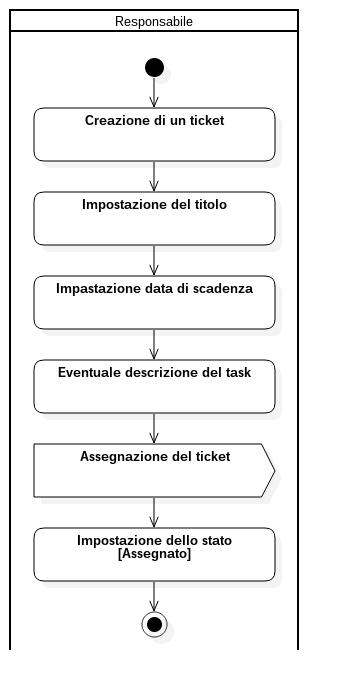
\includegraphics[scale=0.80]{img/creazioneTicket.png}
			\caption{Creazione di un \gl{ticket}}
		\end{figure}
	\paragraph{Aggiornamento di un \gl{ticket}}
	\label{sec:4.1.2.2}
		Ogni membro del gruppo avrà una lista di \gl{ticket} a lui assegnati, su di essi dovrà modificare il tag di stato ogni qual volta uno di questi cambi di stato come descritto dalla sezione 4.1.1.3.1. Nel caso in cui il \gl{ticket} venga \textbf{rifiutato} o venga messo \textbf{in sospeso} è necessario scrivere una motivazione attraverso un commento.
		\begin{figure}
			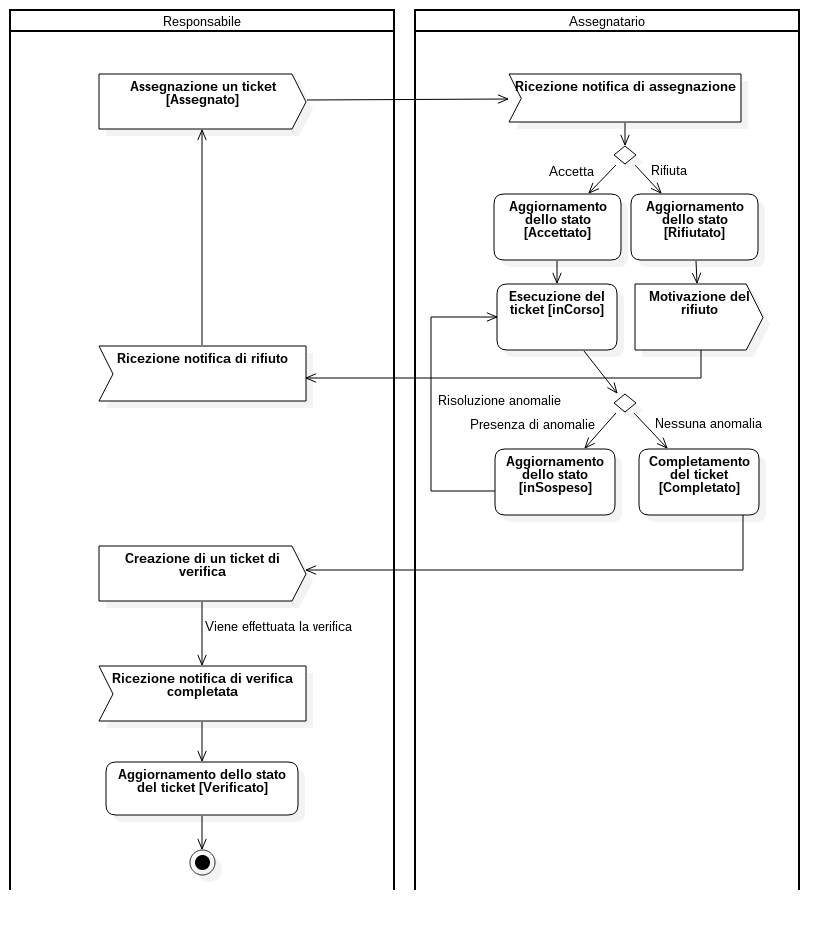
\includegraphics[scale=.53]{img/vitaTicket.png}
			\centering
			\caption{Ciclo di vita di un \gl{ticket}}
		\end{figure}
\subsubsection{Norme}
\label{sec:4.1.3}
	\paragraph{\gl{Repository}}
	\label{sec:4.1.3.1}
		Per la gestione condivisa e per il controllo delle versioni dei file il \gl{team} ha deciso di utilizzare una \gl{repository} fornita dal servizio web \gl{GitHub}.
		\subparagraph{Struttura del \gl{repository}}
		\label{sec:4.1.3.1.1}
			La respository si divide in due cartelle principali:
			\begin{itemize}
				\item \textbf{Codice}: contenente il codice del \gl{progetto}, con struttura ancora da definire;
				\item \textbf{Documenti}: contenente:
				\begin{enumerate}
					\item \textbf{\gl{template}}: con al suo interno i file \file{.sty} e una cartella \textbf{img} contenente le immagini (vedi sezione 3.1.2.1);
					\item \textbf{\gl{script}}: con al suo interno gli \gl{script};
					\item una cartella per ogni \textbf{revisione di avanzamento}, il cui nome è definito dal numero e dalla sigla della revisione, separata da un trattino. Ciascuna di esse è suddivisa in:
					\begin{enumerate}
						\item \textbf{interni}: contenente una cartella per ogni documento interno, con nome, in notazione \gl{CamelCase}, uguale a quello del documento(senza numero di versione);
						\item \textbf{esterni}: contenente una cartella per ogni documento esterno, con nome, in notazione \gl{CamelCase}, uguale a quello del documento(senza numero di versione);
					\end{enumerate}
					Ogni cartella dei documenti ha al suo interno, se necessario, una cartella \textbf{img} contenente le immagini e i diagrammi presenti in quel documento.
				\end{enumerate}
			\end{itemize}
		\subparagraph{Tipi di file e .gitignore}
		\label{sec:4.1.3.1.2}
			All'interno delle cartelle dei documenti saranno presenti solamente i file \file{.tex}, i restanti file ausiliari prodotti da \gl{\LaTeX} sono stati aggiunti a .gitignore e quindi vengono ignorati e resi invisibili da \gl{Git}.
		\subparagraph{Norme sulla \gl{commit}}
		\label{sec:4.1.3.1.3}
			Per rendere effettive le modifiche applicate ai file della \gl{repository} locale è necessario eseguire una \textbf{\gl{commit}}.
			I membri del team sono tenuti ad effettuare una \gl{commit} ogni qual volta venga aggiunta, rimossa o aggiornata una funzionalità oppure una sezione, aggiungendo i file interessati tramite il commando:
			\begin{center}
				\file{\gl{git} add nome\_del\_file.est}
			\end{center}
			ed eseguendo la \gl{commit} tramite il commando:
			\begin{center}
				\file{\gl{git} \gl{commit} -m ``messaggio''}
			\end{center}
			con \file{messaggio} che segua le regole della sezione 3.2.1.
			Infine per rendere effettive le modifiche nel \gl{repository} in remoto eseguire:
			\begin{center}
				\file{\gl{git} \gl{push}}
			\end{center}
		\subparagraph{Messaggi delle \gl{commit}}
		\label{sec:4.1.3.1.4}
			Ogni qual volta venga eseguita una \file{\gl{commit}} è obbligatorio inserire un breve messaggio con la spiegazione
			delle modifiche apportate; il messaggio deve iniziare con:
			\begin{itemize}
				\item \textbf{Add:} se vengono aggiunte funzionalità o sezioni;
				\item \textbf{Remove:} se vengono tolte funzionalità o sezioni;
				\item \textbf{Update:} se vendono aggiornate funzionalità o sezioni;
				\item \textbf{Fix:} se viene sistemato un bug noto;
			\end{itemize}
			deve seguire una descrizione sintetica in lingua italiana delle modifiche apportate.
\subsubsection{Strumenti}
\label{sec:4.1.4}
	\paragraph{Sistema operativo}
	\label{sec:4.1.4.1}
		Non ci sono restrizioni riguardo l'utilizzo di un sistema operativo: ogni membro del team può utilizzare quindi il sistema operativo che preferisce; in ogni caso, è tenuto a rendere il materiale \gl{prodotto} \textbf{completamente} compatibile su tutte le piattaforme.
	\paragraph{Condivisione}
	\label{sec:4.1.4.2}
		Il servizio da utilizzare per i documenti informali è \gl{Google Drive}.
		All'interno di questo \gl{repository} vanno caricati documenti che:
		\begin{itemize}
			\item non necessitano di controllo di versione;
			\item necessitano di essere modificati contemporaneamente da più persone; infatti \gl{Google Drive} permette la modifica di un documento in contemporanea: in questo modo non ci saranno conflitti.
		\end{itemize}
		È possibile anche condividere link o manuali utili per la formazione del team. Si può installare \gl{Google Drive} sul proprio PC: i file così potranno essere disponibili anche offline e sincronizzare il contenuto della cartella ad ogni aggiornamento.
	\paragraph{Gestione}
	\label{sec:4.1.4.3}
		\begin{itemize}
			\item \textbf{Ticket}: per la gestione dei \gl{ticket} è stato scelto di utilizzare \gl{Asana}; per la gestione dei \gl{ticket}, si rimanda alla sezione 4.1.2.1;
			\item \textbf{Requisiti e casi d'uso}: per il tracciamento dei requisiti si utilizzerà \gl{Trender}. Per quanto riguarda la rappresentazione dei casi d'uso l'editor consigliato è \gl{Star UML}; %vedi sezione requisiti 
			\item \textbf{Scadenze}: \gl{Google Calendar} verrà utilizzato per segnare le scadenze del gruppo; si riceverà una notifica su \gl{Slack} trenta minuti prima dell'evento;
			\item \textbf{Progetto}: per la realizzazione dei grafici di \gl{Gantt} è stato impiegato il programma \gl{GanttProject}.
		\end{itemize}

\end{document}